\section{Grundlagen}
\label{raeumliche_grundlagen}

Für die Definition eines räumlichen Faltungsoperators auf Graphen werden spezielle Konstrukte der Graphentheorie benötigt, die im Folgenden vorgestellt werden.

\paragraph{Färbung von Knoten}
\label{faerbung_von_knoten}

Eine \emph{Knotenfärbung} $\gls{l}$ ist eine Funktion $\gls{l} \colon \gls{V} \to \gls{C}$ auf den Knoten eines Graphen \gls{G}, die jedem Knoten in \gls{V} eine \emph{Farbe} einer endlich abzählbaren Menge $\gls{C} \subseteq \gls{R}$ zuordnet~\cite{patchy}.
Mit Hilfe der Knotenfärbung lässt sich folglich eine Ordungsrelation $>_{\gls{l}}$ auf der Knotenmenge von \gls{G} definieren, wobei $\gls{v}_i >_{\gls{l}} \gls{v}_j$ genau dann, wenn $\gls{l}\left(\gls{v}_i\right) < \gls{l}\left(\gls{v}_j\right)$~\cite{patchy}.
Falls \gls{l} weiterhin injektiv ist, so spricht man von einer \emph{totalen Ordnung} und die Knoten $\gls{v} \in \gls{V}$ können insbesondere so permutiert werden, dass sie die Ordnung von $>_{\gls{l}}$ respektieren~\cite{patchy}.

Beispiele für eine Knotenfärbung sind Metriken, die die Wichtigkeit der einzelnen Knoten beschreiben.
Eine naive Metrik dafür ist \zB{} der Knotengrad \gls{degree} \bzw{} \gls{d}, der die \emph{Zentralität} der Knoten beschreibt~\cite{patchy}.
Komplexere Metriken für die Zentralität der Knoten sind unter anderem die Nähe, die Betweenness-Zentralität sowie die Eigenvektorzentralität~\cite{patchy, centrality}.
Letztere ist eng mit dem \emph{PageRank}-Algorithmus von Google verwandt~\cite{centrality}.
Die \emph{Nähe} (\engl{} \emph{Closeness})
\begin{equation*}
  c\left(\gls{v}\right) \coloneqq \frac{1}{\sum_{\gls{v}_i \in \gls{V}, \gls{v} \neq \gls{v}_i} \gls{s}\left(\gls{v}, \gls{v}_i\right)}
\end{equation*}
ist ein Maß für die durchschnittliche Länge zwischen einem Knoten und allen weiteren Knoten in \gls{V}~\cite{centrality}.
Je \emph{näher} ein Knoten sich an der Knotenmenge befindet, als desto zentraler gilt er.
Die \emph{Betweenness-Zentralität} eines Knotens $\gls{v} \in \gls{V}$ ist über
\begin{equation*}
  c\left(\gls{v}\right) \coloneqq \sum_{\gls{v}_i \neq \gls{v} \neq \gls{v}_j} \frac{\kappa_{ij}\left(\gls{v}\right)}{\kappa_{ij}}
\end{equation*}
definiert, wobei $\kappa_{ij} \in \gls{N}$ die Anzahl an kürzesten Pfaden von $\gls{v}_i$ nach $\gls{v}_j$ angibt und $\kappa_{ij}\left(\gls{v}\right) \in \gls{N}$ die Anzahl dieser Pfade beschreibt, die durch \gls{v} führen~\cite{centrality}.
Nach der Methode der \emph{Eigenvektorzentralität} gilt ein Knoten als umso wichtiger, je wichtiger seine Nachbarknoten sind~\cite{centrality}.
Sie ist definiert über
\begin{equation*}
  c\left(\gls{v}\right) = \frac{1}{\gls{lambda}} \sum_{\gls{v}_i \in \gls{Neighbor}\left(\gls{v}\right)} c\left(\gls{v}_i\right),
\end{equation*}
wobei $\gls{lambda} \in \gls{R}$.
Mit der Darstellung der Eigenvektorzentralität $c \colon \gls{V} \to \gls{R+}$ als Vektor $\ve{c} \in \gls{R+}^N$ und \gls{G} als ungewichtete Adjazenzmatrix $\gls{A} \in {\left\{0,1\right\}}^{N \times N}$ kann die Bestimmung von \gls{lambda} \bzw{} \ve{c} als Eigenwertproblem $\gls{A}\ve{c} = \gls{lambda}\ve{c}$ aufgefasst werden.
Dann beschreibt der größte Eigenwert \gls{lambda} die Eigenvektorzentralität der Knoten über dessen Eigenvektor \ve{c}~\cite{centrality}.

\paragraph{Isomorphie und kanonische Ordnung}
\label{isomorphie_und_kanonische_ordnung}

Seien $\gls{G}_1 = \left(\gls{V}_1, \gls{E}_1\right)$ und $\gls{G}_2 = \left(\gls{V}_2, \gls{E}_2\right)$ zwei Graphen mit der gleichen Anzahl an Knoten, \dhe{} $\left|\gls{V}_1\right| = \left|\gls{V}_2\right|$.
Dann heißt eine bijektive Abbildung $p \colon \gls{V}_1 \to \gls{V}_2$ \emph{Isomorphismus} zwichen $\gls{G}_1$ und $\gls{G}_2$, falls $\left(\gls{v}_i, \gls{v}_j\right) \in \gls{E}_1$ \gdw{} $\left(p\left(\gls{v}_i\right), p\left(\gls{v}_j\right)\right) \in \gls{E}_2$~\cite{nauty}.
Zwei Graphen sind genau dann \emph{isomorph} zueinander, wenn ein Isomorphismus zwischen ihnen existiert.
Die Komplexität zur Bestimmung der Isomorphie zweier Graphen liegt in NP, wobei nicht bekannt ist, ob sie in P enthalten oder NP-vollständig ist~\cite{patchy}.

Die Komposition mehrerer Isomorphismen ist ebenfalls ein Isomorphismus~\cite{nauty}.
Die Menge aller Isomorphismen (zuzüglich der identischen Abbildung, die die Knoten auf sich selber abbildet) heißt die \emph{Isomorphismenklasse} des Graphen~\cite{nauty}.

Eine \emph{kanonische Ordnung} eines Graphen $\gls{G} = \left(\gls{V}, \gls{E}\right)$ ist ein Graph $\gls{G}^{\prime} = \left(\gls{V}^{\prime}, \gls{E}^{\prime}\right)$ mit einer eindeutigen Ordnung seiner Knoten $\gls{V}^{\prime}$, der isomorph zu \gls{G} ist und seine gesamte Isomorphismenklasse repräsentiert~\cite{patchy}.
Zwei Graphen sind insbesondere genau dann zueinander isomorph, wenn ihre kanonischen Ordnungen übereinstimmen~\cite{nauty}.
Abbildung~\ref{fig:kanonische_ordnung} illustriert das Prinzip der kanonischen Ordnung anhand zwei einfach gewählter zueinander isomorpher Graphen.
\begin{figure}[t]
\centering
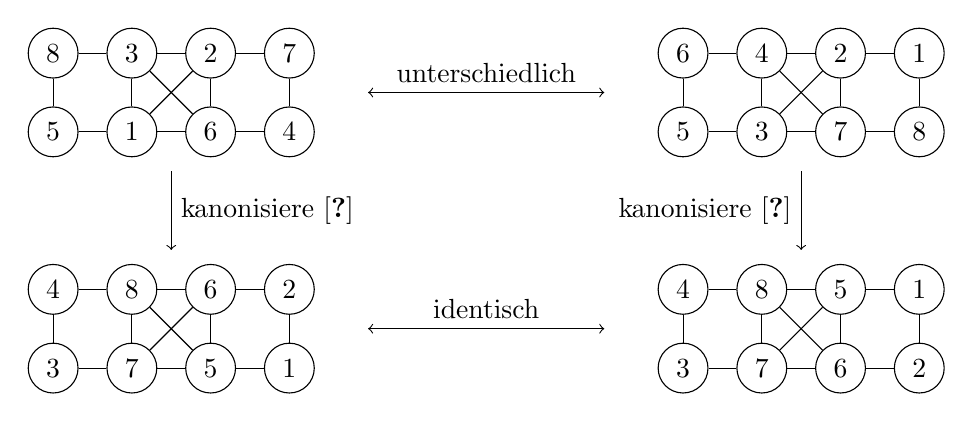
\begin{tikzpicture}
  \tikzstyle{node}=[circle,draw, minimum width=18pt, inner sep=0pt, fill=white]

  \node[node] (a1) at (0, 4) {$8$};
  \node[node] (a2) at (1, 4) {$3$};
  \node[node] (a3) at (2, 4) {$2$};
  \node[node] (a4) at (3, 4) {$7$};
  \node[node] (a5) at (0, 3) {$5$};
  \node[node] (a6) at (1, 3) {$1$};
  \node[node] (a7) at (2, 3) {$6$};
  \node[node] (a8) at (3, 3) {$4$};

  \path (a1) edge (a2);
  \path (a1) edge (a5);
  \path (a2) edge (a3);
  \path (a2) edge (a6);
  \path (a2) edge (a7);
  \path (a3) edge (a4);
  \path (a3) edge (a6);
  \path (a3) edge (a7);
  \path (a4) edge (a8);
  \path (a5) edge (a6);
  \path (a6) edge (a7);
  \path (a7) edge (a8);

  \node[node] (b1) at (0, 1) {$4$};
  \node[node] (b2) at (1, 1) {$8$};
  \node[node] (b3) at (2, 1) {$6$};
  \node[node] (b4) at (3, 1) {$2$};
  \node[node] (b5) at (0, 0) {$3$};
  \node[node] (b6) at (1, 0) {$7$};
  \node[node] (b7) at (2, 0) {$5$};
  \node[node] (b8) at (3, 0) {$1$};

  \path (b1) edge (b2);
  \path (b1) edge (b5);
  \path (b2) edge (b3);
  \path (b2) edge (b6);
  \path (b2) edge (b7);
  \path (b3) edge (b4);
  \path (b3) edge (b6);
  \path (b3) edge (b7);
  \path (b4) edge (b8);
  \path (b5) edge (b6);
  \path (b6) edge (b7);
  \path (b7) edge (b8);

  \node[node] (c1) at (8,  4) {$6$};
  \node[node] (c2) at (9,  4) {$4$};
  \node[node] (c3) at (10, 4) {$2$};
  \node[node] (c4) at (11, 4) {$1$};
  \node[node] (c5) at (8,  3) {$5$};
  \node[node] (c6) at (9,  3) {$3$};
  \node[node] (c7) at (10, 3) {$7$};
  \node[node] (c8) at (11, 3) {$8$};

  \path (c1) edge (c2);
  \path (c1) edge (c5);
  \path (c2) edge (c3);
  \path (c2) edge (c6);
  \path (c2) edge (c7);
  \path (c3) edge (c4);
  \path (c3) edge (c6);
  \path (c3) edge (c7);
  \path (c4) edge (c8);
  \path (c5) edge (c6);
  \path (c6) edge (c7);
  \path (c7) edge (c8);

  \node[node] (d1) at (8,  1) {$4$};
  \node[node] (d2) at (9,  1) {$8$};
  \node[node] (d3) at (10, 1) {$5$};
  \node[node] (d4) at (11, 1) {$1$};
  \node[node] (d5) at (8,  0) {$3$};
  \node[node] (d6) at (9,  0) {$7$};
  \node[node] (d7) at (10, 0) {$6$};
  \node[node] (d8) at (11, 0) {$2$};

  \path (d1) edge (d2);
  \path (d1) edge (d5);
  \path (d2) edge (d3);
  \path (d2) edge (d6);
  \path (d2) edge (d7);
  \path (d3) edge (d4);
  \path (d3) edge (d6);
  \path (d3) edge (d7);
  \path (d4) edge (d8);
  \path (d5) edge (d6);
  \path (d6) edge (d7);
  \path (d7) edge (d8);

  \draw[<->] (4,   3.5) -- node[above] {unterschiedlich}          (7,   3.5);
  \draw[<->] (4,   0.5) -- node[above] {identisch}                (7,   0.5);
  \draw[->]  (1.5, 2.5) -- node[right] {kanonisiere~\cite{nauty}} (1.5, 1.5);
  \draw[->]  (9.5, 2.5) -- node[left]  {kanonisiere~\cite{nauty}} (9.5, 1.5);

\end{tikzpicture}
\caption[Kanonische Ordnung]{Illustration zweier isomorpher Graphen (oben), die jedoch nicht identisch sind (\zB{} sind die Knoten $1$ und $5$ im linken Graphen adjazent, aber nicht im rechten).
Der Prozess zur Bestimmung einer kanonischen Ordnung sorgt dafür, dass zwei Graphen eine identische Knotenabbildung erhalten, falls sie isomorph zueinander sind (unten).
Die Kanten der Graphen verweisen jeweils auf die gleichen Indizes, auch wenn sich die Darstellung \bzw{} Position der Knoten unterscheidet.}
\label{fig:kanonische_ordnung}
\end{figure}


Ein Isomorphismus \bzw{} eine kanonische Ordnung kann ebenfalls eine Knotenfärbung \gls{l} berücksichtigen, indem Knoten durch einen Isomorphismus nur auf Knoten der gleichen Farbe abgebildet werden dürfen~\cite{nauty}.
Das reduziert die Menge der verfügbaren Isomorphismenklassen und insbesondere die Komplexität ihrer Berechnung.
Zur Berechnung der Isomorphismenklassen und der kanonischen Ordnung, auch unter Berücksichtigung einer Knotenfärbung, zeichnet sich das Programm \texttt{nauty} aufgrund dessen bemerkenswerter Berechnungslaufzeit aus (\vgl{}~\cite{nauty}).
